\chapter{Linking ecosystem size distributions to environmental disturbance regimes}

\section{Introduction and Justification}

Forests are fundamental to Earth's biosphere, regulating carbon, energy, and water cycles at planetary scales. They store over $40\%$ of terrestrial carbon and drive more than half of the net primary productivity \cite{bonan_forests_2008, pan_large_2011}. Terrestrial vegetation makes up the majority of biomass on earth, fueling virtually every biochemical process in the biosphere \cite{bar-on_biomass_2018}. Despite their ecological and societal importance, forests remain a significant source of uncertainty in climate projections. This is mainly due to the paucity of large-scale data capable of constraining carbon turnover rates and predicting responses to disturbance \cite{doughty_tropical_2023, friedlingstein_global_2023, pugh_understanding_2020}. To improve climate models, we must develop scalable, predictive approaches for assessing forest resilience and disturbance.

Due to their ecological and societal value, forests have a long history of meticulous monitoring; ranging from long-term field studies to national inventories. Forest monitoring has evolved from field-based inventories to sophisticated remote sensing approaches, promising global coverage with increasing temporal and spatial resolution. These efforts have provided critical data for carbon budgeting and revealed patterns in forest structure, biogeography, and demographics \cite{duncanson_assessing_2015,friedlingstein_global_2023}. In addition, remote sensing is widely adopted into inventory and monitoring strategies, promising unprecedented spatial coverage and temporal resolution \cite{fassnacht_remote_2024, duncanson_aboveground_2022}. However, despite these advances, precise quantification of disturbance remains challenging (Gao et al., 2020). Current vegetation models often rely on historical correlations, but nonlinear feedbacks between forest biota and the Earth system likely introduce tipping points that undermine conventional projections \cite{dietz_economic_2021, lenton_environmental_2013}. There is a pressing need for scalable and reproducible methods that link large-scale tree dynamics to underlying environmental processes, including anthropogenic change. 

A key concern in existing vegetation dynamic models is the reliance on historical correlations of net carbon assimilation with numerous biotic and abiotic factors \cite{allen_underestimation_2015, barnes2022a}. For example, the Amazon rainforest’s response to severe drought events has been shown to vary considerably \cite{anderegg_divergent_2020, saleska_amazon_2007}. Recent work has demonstrated that incorporating information about local environmental conditions (e.g. topography and water table depth), as well as focal functional traits, explains a significant portion of the residual variation \cite{chen_amazon_2024, signori-muller_non-structural_2021, tavares_basin-wide_2023}. However, in most instances it is a priori unknown which biotic and abiotic factors will be important, making it difficult to generalize across forest ecosystems. 

Anticipating the effects of particular stressors on tree communities is particularly challenging due to the numerous feedbacks. Ecosystem responses to novel environmental regimes largely depend on their historic exposure to different disturbance types and existing functional variation \cite{renes_disturbance_2020, hoffmann_environmental_2000}. A corollary of this is that not all species will react proportionally to the same conditions. Thus, community resilience can only be fully quantified through large-scale trends in species abundance distributions \cite{loreau2010a, arnoldi_how_2018}. Distribution patterns have been used to identify susceptible ecosystems in numerous studies \cite{chaalali_species_2016, padfield_linking_2018, pecl_biodiversity_2017} and have proven to be especially insightful when paired with process-based modeling \cite{dakos2011a}. 

Forests across the globe display an astonishing diversity of functional traits, many of which are closely related to environmental conditions \cite{lopez_coordination_2021, reich2014a}. A few traits vary so consistently across large climatic and taxonomic ranges to indicate the dominance of highly conserved physiological constraints \cite{delong_shifts_2010, hatton2019a, wright2004a}. Among these, body size (i.e. tree height) is perhaps the most well-established due to its close association with organismal metabolic rate, as well as its implications for ecosystem-wide energy fluxes \cite{allen2005a, brown2004a, savage_sizing_2008}. Beyond its relationship with energetic expenditure, the importance of tree size is made apparent through robust structural and functional allometries \cite{chave_improved_2014, goodman_importance_2014, niklas_invariant_2001}. Indeed, numerous studies have leveraged size-abundance distributions to assess the general health and functionality of various biological systems \cite{chaalali_species_2016, guo_size_2022, spanbauer_body_2016}. However, despite the widespread use of allometric scaling in estimating aboveground carbon sequestration, its implications for forest resilience and robustness remain largely unexplored. 

Interpreting size-abundance distributions is facilitated when framed within theoretical models of size-structured vegetation growth. These models divide trees into size classes and assume that growth is given by a combination of resource acquisition, basal metabolism, mortality, and competition. A general formulation is given by the Von Foerster equation, where the change in abundance of size class, defined as all trees of height $h$, ($h_{k-1} \leq h \leq h_{k} $), is given by the growth of smaller size classes ($N_{k-1}$) at rate $\dot{h}_{k-1}$, minus growth into larger trees ($\dot{h}_{k}$), minus a mortality term, $\mu_{k}$. 

\begin{equation}
    \dfrac{dN_{k}}{dt} = \dfrac{N_{k-1}\dot{h}_{k-1}(R) - N_{k}\dot{h}_{k}(R)}{h_{k}-h_{k-1} }  - \mu_{k}N_{k}
\end{equation}

In principle size classes can be made arbitrarily small, rendering a system of partial differential equations. Detailed analyses of such continuous size models have been previously carried out \cite{enquist_scaling_2024, lee_growth_2021, moorcroft_method_2001,  odwyer_integrative_2009}, yielding expected equilibrium size distributions and subsequent deviations caused by different forms of perturbation. If we part from the most basic set of assumptions, that is, that growth and mortality scale as power functions of height ($g(h) = ah^{c} $ and $m(h)=rh^{b} $ ) the resulting, normalized steady state distribution (henceforth SSD) is given by a Weibull distribution \cite{muller-landau_comparing_2006}.

\begin{equation}
    P(h) = \dfrac{1}{N_{0}} h^{-c} \exp{\left[ \dfrac{-ah^{1+b-c}}{r(1 + b -c )} \right]} 
\end{equation}

The generality of size-structured frameworks has lent itself to a wide range of applications; in particular its adoption in Earth System Models (ESM) such as the DOE’s ELM-FATES which is derived from the Ecosystem Demography Model \cite{fisher_taking_2015, moorcroft_method_2001}. ESMs have likewise been used to simulate and inform understanding of forest disturbance dynamics \cite{shi_functionally_2024}. Though the granularity of complex models such as FATES is indispensable to generate fine-scale predictions, there is a need for coarse-grained approaches that allow us to assess general patterns of ecosystem structure, and identify large-scale signatures of disturbance. 

\section{Approach and Methods}

Here, I propose a novel approach for quantifying forest robustness and resilience based on allometric models of vegetation growth and size-abundance distributions inferred from remote sensing. This research consists of three components: (1) Mapping global forest height distributions using GEDI LiDAR waveforms and SAR tomography. (2) Using size-abundance distributions and climate data to parameterize size-structured vegetation models and establish baseline expectations. (3) Comparing modeled predictions to forests with known disturbance regimes (i.e. managed forests) to generate quantitative disturbance profiles. 

\subsection{Mapping global forest height distributions with remote sensing} \label{task1}

Advancements in remote sensing now allow for the reconstruction of forest structure with increasing accuracy. In particular, GEDI LiDAR has proven to be especially valuable for above-ground biomass estimation, especially when paired with other remote sensing tools and calibrated with field data \cite{chi_national_2015, crockett_structural_2023, potapov_mapping_2021}. Although uncertainties exist in tree height estimation, recent studies indicate that GEDI can accurately capture normalized height frequency distributions which better reflects size structure \cite{tan_exploring_2024}. Specifically, Ngo et al., \cite{ngo_tropical_2022} demonstrated that GEDI waveforms accurately characterized the vertical structure of tropical forests when combined with P-band synthetic aperture radar (SAR) tomography (Figure 2).

I will use forest inventory data to calibrate a pipeline that infers height frequency distributions from GEDI waveforms in conjunction with existing SAR tomography datasets, such as TanDEM-X, TerraSAR-X and ESA’s upcoming BIOMASS mission. We will borrow from recently developed remote sensing methods and leverage existing models that estimate size structure from field-based measurements \cite{ngo_tropical_2022, ramachandran_evaluation_2021}. 
The first stage of the pipeline will identify appropriate datasets with which to train and validate the inference procedure. The selection process will be based on criteria laid out by Crockett et al. \cite{crockett_structural_2023}, emphasizing the requirement that forest plots be sampled from 2017 and that they be at least 90\% forested. Currently this includes at least 1796 FIA plots and will likely extend to similar inventory data so long as it contains diameter at breast height (DBH) measurements. DBH measurements will be used to predict stand-level diameter distributions using a Maximum Entropy model described in \cite{chen_stand_2019}.

Field-based diameter distributions will then be used to train and evaluate models that predict size-abundance distributions from GEDI waveforms and SAR backscatter profiles. Two main modeling approaches will be compared: deep learning with convolutional neural networks based on the FORMS model \cite{schwartz_forms_2023}, and random forest regression coupled with Monte Carlo simulation \cite{li_aboveground_2022}. Both of these approaches have shown promising results in estimating above ground biomass from remote sensing data, and we expect similar performance when estimating size distributions.

\subsection{Baseline Predictions in Pristine Forests}
\label{task2}

This portion of the chapter will use data from pristine forests to parameterize a general model of vegetation growth. The purpose of this is to provide threshold expectations for how climate and biogeography impact forest height structure in the absence of long-term perturbations. Environmental parameters will be constrained through historical average precipitation and photon flux densities derived from climate models. I present a slightly modified version of the Von Foerster model to explicitly incorporate stochasticity.

\begin{figure}[ht!]
    \centering
    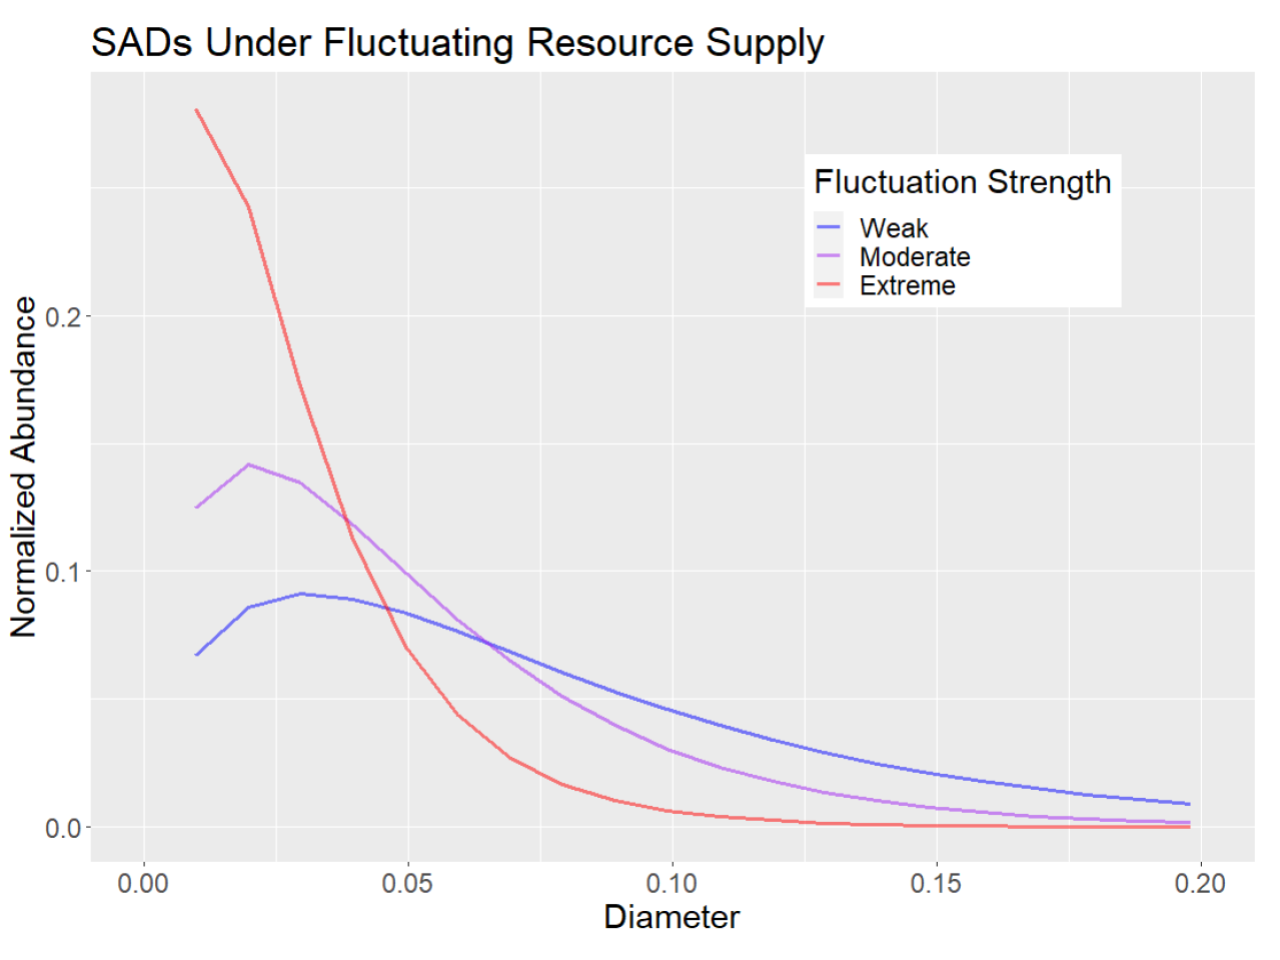
\includegraphics[width=0.8\textwidth]{figures/SAD_fig.png} 
    \caption{Size-abundance distributions from an early implementation of the size-strucutured model. This proof of principle illustrates how resource fluctuations shape the SAD under different resource fluctuation regimes. The distribution shifts towards smaller trees as fluctuations become more severe.}
    \label{fig:SAD}
\end{figure} 

\begin{equation}
    \dfrac{\partial N(h, t)}{\partial t} = \dfrac{\partial}{\partial h} [N(h, t)\dot{h}(h)] - N(h, t)\left[\mu(h, t) + \int_{h_{0}}^{\infty}\alpha(h, h^{\prime})N(h^{\prime}, t)dh^{\prime} \right]
\end{equation}

The first term on the right-hand side describes the average growth of the size distribution in ideal, resource-replete conditions. The following term quantifies how environmental conditions and biotic interactions impact forest-wide variation in growth rates. Hence, assuming that fluctuations in mortality and resource supply follow a given functional form, the SSD can be related to the prevalence of disturbance and competitive interactions. Furthermore, assessing the system’s susceptibility to acute and chronic perturbations can be straightforward through analytical and numerical means (Figure 3). Mortality, $\mu(h, t)$, can be represented as a stochastic process.

\begin{equation}
     \mu(h, t) = \mu_{W}(h)dW
\end{equation}

The size dependence of $\mu_{W}(h)$ considers that disturbance events may preferentially impact trees of a particular height. The effect of fluctuating resources can be incorporated as a modification to the basal growth rate which accounts for resource limitation.
\begin{equation}
    \dot{h}(t, h) =g_{0}h^{c} \dfrac{V(h)\rho(t)}{V(h)\rho(t) + Q_{0}(h)K(h)} - \mu_{o}h^{b} ,  \quad K(h) =\dfrac{g_{0}h^{c}}{\mu_{0}h^{b}} - 1 
\end{equation}

Here $V(h)$ represents a harvesting volume and $Q_{0}(h)$ is the basal metabolic demand for a tree of a given size. Assuming that $V(h)$ is proportional to the radial extent of the root system and $Q_{0}(h)$ is set by maintenance metabolism,  harvesting volume and basal demand can be defined as power functions of $h$ as per \cite{kempes2011a, niklas_growth_2004}. Additionally, $\rho(t)$ is the time-fluctuating density of resources with mean $\rho_{0}$.

The time dependence denoted by $\chi(t)$ can be modeled as colored noise based on observed supply time-series, such as the one provided by the standardized precipitation evapotranspiration index (SPEI) \cite{begueria_standardized_2014}. Finally, we assume that competition is inversely proportional to an exponent of height, requiring that competitive burden decrease as trees get taller.

\begin{equation}
    \beta_{0}h^{-\alpha} \sim \int_{h_{0}}^{\infty} \alpha(h, h^{\prime})N(h^{\prime})dh^{\prime}, \quad \rho(t) = \dfrac{\rho_{0}}{\chi(t)}
\end{equation}


Having defined the system in this manner and assuming that intact forests are dominated by resource supply and metabolic demand constrains nearly all parameters through robust allometric relationships and climate. Hence, the fitting procedure is only concerns the interaction structure of the underlying vegetation ($\beta_{0}h^{-\alpha}$).

\subsection{Characterizing Disturbance From Deviations in Managed Forests}
\label{task3}

Using results from \ref{task2}, I will analyze forests with biogeographic adjacency but varying disturbance regimes. The premise is that forests with similar interaction structure and climate should exhibit comparable size-abundance distributions in the absence of disturbance. By comparing disturbed forests to baseline expectations, I will quantify the impact of different disturbance types. This involves (1) Identifying forests with independently quantifiable, above baseline mortality rates; and (2) using inferred height profiles to parameterize added mortality.



